\chapter{Pavlovian learning}


Form of prediction learning that aims to learn stimulus-outcome associations:
\begin{itemize}
    \item When a reinforcer is likely to occur.
    \item Which stimuli tend to precede a reinforcer.
\end{itemize}
This allows the animal to emit a response in anticipation of a reinforcer.

Pavlovian learning works as follows:\\
\begin{minipage}{0.58\linewidth}
    \begin{enumerate}[label=\alph*.]
        \item A stimulus that has no meaning to the animal will result in \ac{nr}.
        \item An \ac{us} (i.e. a reinforcer) generates an \ac{ur}.
        \item Learning happens when a reinforcer is paired with a non-relevant stimulus.
        \item The learned \ac{cs} generates a \ac{cr}.
    \end{enumerate}
\end{minipage}
\begin{minipage}{0.4\linewidth}
    \raggedleft
    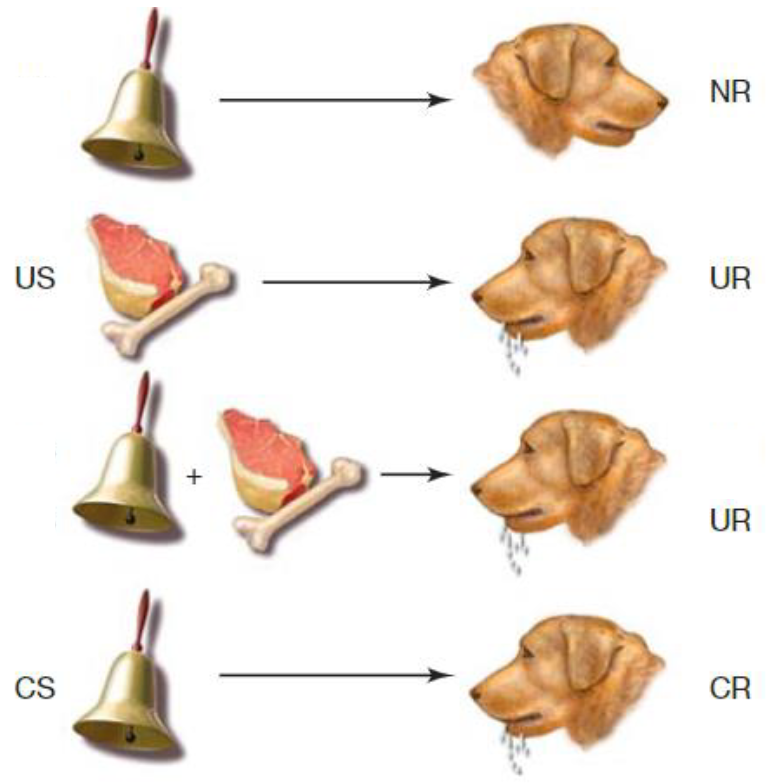
\includegraphics[width=0.9\linewidth]{./img/pavlovian_example.png}
\end{minipage}\\

An outcome can be:
\begin{descriptionlist}
    \item[Appetitive] Something considered positive.
    \item[Aversive] Something considered negative.
\end{descriptionlist}

The learned \acl{cr} can be:
\begin{descriptionlist}
    \item[Behavioral] Associated to the startle response (i.e. reflex in response to a sudden stimulus).
    \item[Physiological] Associated to the autonomic system.
    \item[Change in subjective response] 
\end{descriptionlist}

\begin{remark}
    Pavlovian learning has its foundations in behaviorism: the brain starts as a blank slate and only observable behaviors can be studied.
\end{remark}



\section{Types of reinforcement}

There are two types of learning:
\begin{descriptionlist}
    \item[Continuous reinforcement] \marginnote{Continuous reinforcement}
        The \acl{cs} is reinforced every time the \acl{us} occurs.
        \begin{remark}
            More effective to teach a new association.
        \end{remark}

    \item[Partial reinforcement] \marginnote{Partial reinforcement}
        The \acl{cs} is not always reinforced.
        \begin{remark}
            Learning is slower but the \acl{cr} is more resistant to extinction.
        \end{remark}
\end{descriptionlist}



\section{Learning flexibility}

\begin{description}
    \item[Acquisition] \marginnote{Acquisition}
        The probability of occurrence of a \acl{cr} increases if the \acl{cs} is presented with the \acl{us}.
        
    \item[Extinction] \marginnote{Extinction}
        The probability of occurrence of a \acl{cr} decreases if the \acl{cs} is presented alone.
\end{description}

\begin{remark}
    Extinction does not imply forgetting.
    After an association between \ac{cs} and \ac{us} is made, 
    extinction consists of creating a second association with inhibitory effects that overrides the existing association.

    The extinct association can return in the future
    (this is more evident when the context is the same as the acquisition phase).
\end{remark}

\begin{figure}[H]
    \centering
    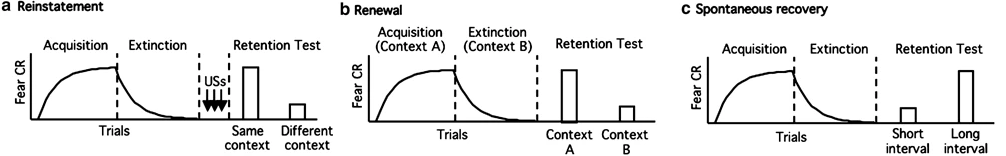
\includegraphics[width=0.95\linewidth]{./img/pavlovian_extinction.png}
    \caption{Example of acquisition, extinction, and \ac{cr} return}
\end{figure}

\begin{description}
    \item[Generalization] \marginnote{Generalization} 
        A new stimulus that is similar to a learned \acl{cs} can elicit a \acl{cr}.
\end{description}

\begin{casestudy}[Aplysia Californica] \phantom{}\\
    \begin{minipage}{0.8\linewidth}
        \begin{enumerate}
            \item Before conditioning, a stimulus to the siphon of an aplysia californica results in a weak withdrawal of the gill.
            \item During conditioning, a stimulus to the siphon is paired with a shock to the tail which results in a large withdrawal of the gill.
            \item After conditioning, a stimulus to the siphon alone results in a large withdrawal response.
        \end{enumerate}
    \end{minipage}
    \begin{minipage}{0.18\linewidth}
        \centering
        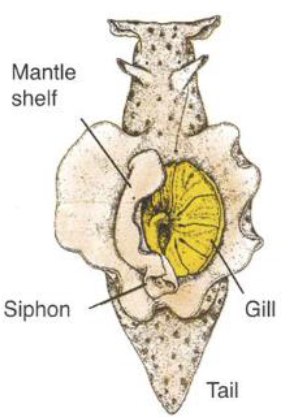
\includegraphics[width=\linewidth]{./img/aplysia.png}
    \end{minipage}

    \begin{figure}[H]
        \centering
        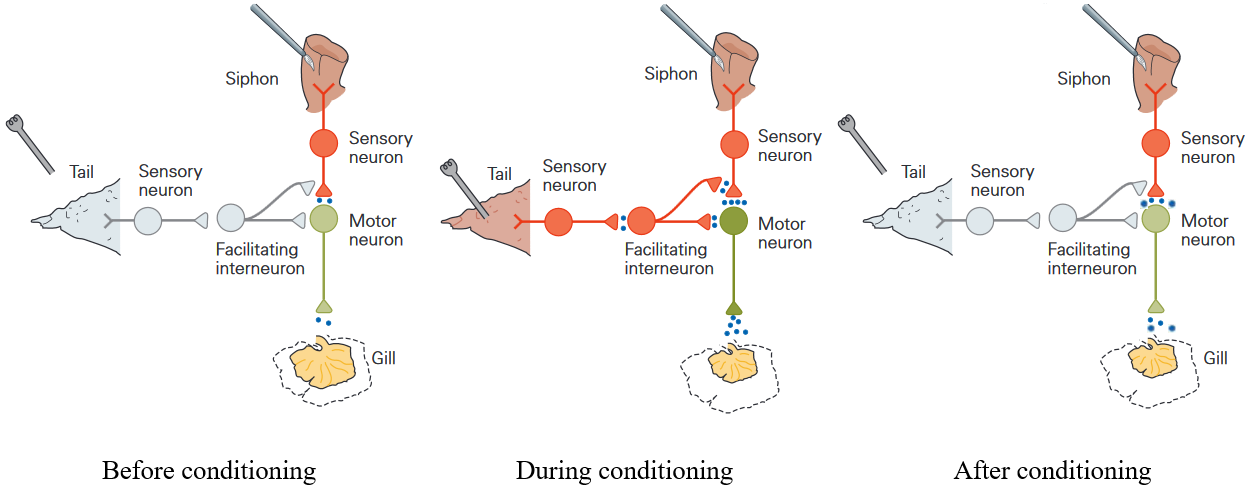
\includegraphics[width=0.85\linewidth]{./img/gill_pavlovian.png}
        \caption{Conditioning process}
    \end{figure}

    The learned response lasts for days.
    It can be observed that without training, the response disappears faster.

    \begin{figure}[H]
        \centering
        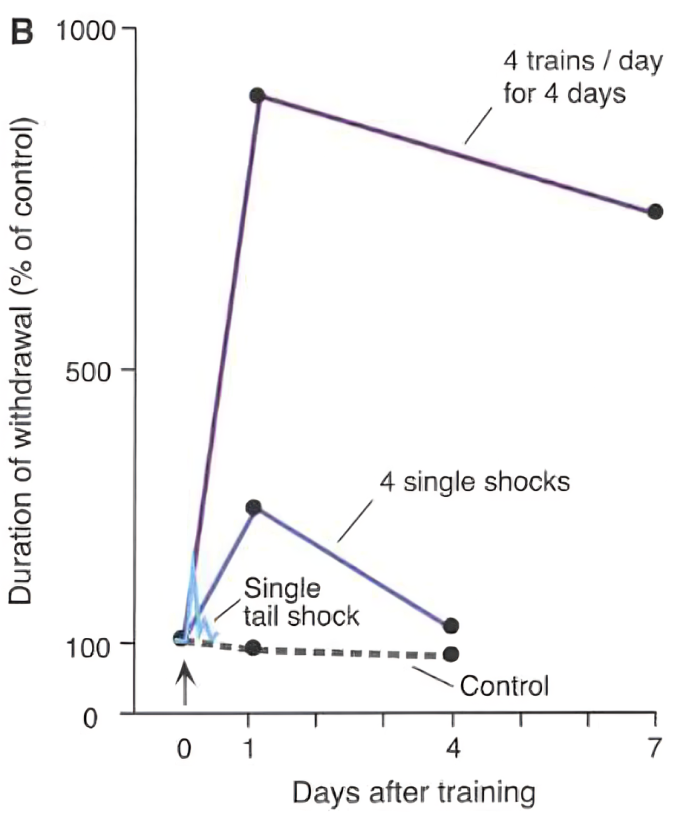
\includegraphics[width=0.3\linewidth]{./img/gill_pavlovian_graph.png}
        \caption{Withdrawal response decay}
    \end{figure}
\end{casestudy}

\begin{remark} \marginnote{Amygdala in Pavlovian learning}
    In mammals, aversive Pavlovian conditioning involves the amygdala.
    The \ac{cs} and \ac{us} are relayed from the thalamus and the cerebral cortex to the amygdala, 
    which in turn connects to various motor responses such as:
    \begin{descriptionlist}
        \item[Central gray region (CG)] Controls the freezing behavior.
        \item[Lateral hypothalamus (LH)] Controls autonomic responses.
        \item[Paraventricular hypothalamus (PVN)] Controls stress hormones.
    \end{descriptionlist}

    \begin{figure}[H]
        \centering
        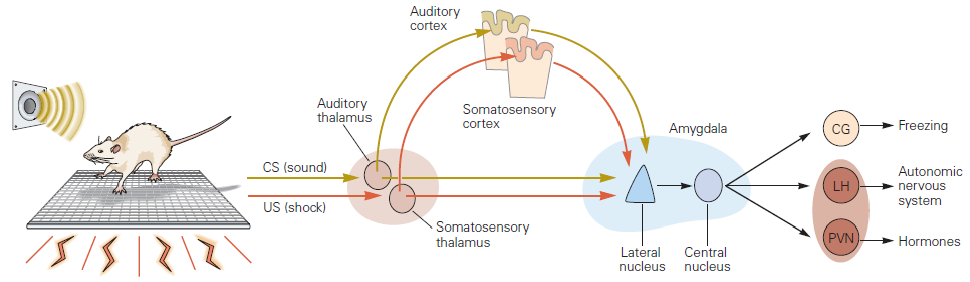
\includegraphics[width=0.9\linewidth]{./img/amygdala_pavlovian.png}
        \caption{Neural circuits during aversive conditioning}
    \end{figure}
\end{remark}



\section{Memory}
\marginnote{Memory}

Memory is vulnerable to alteration.
Once reactivated, the subsequent reconsolidation phase might store a modified version of the memory.

\begin{figure}[H]
    \centering
    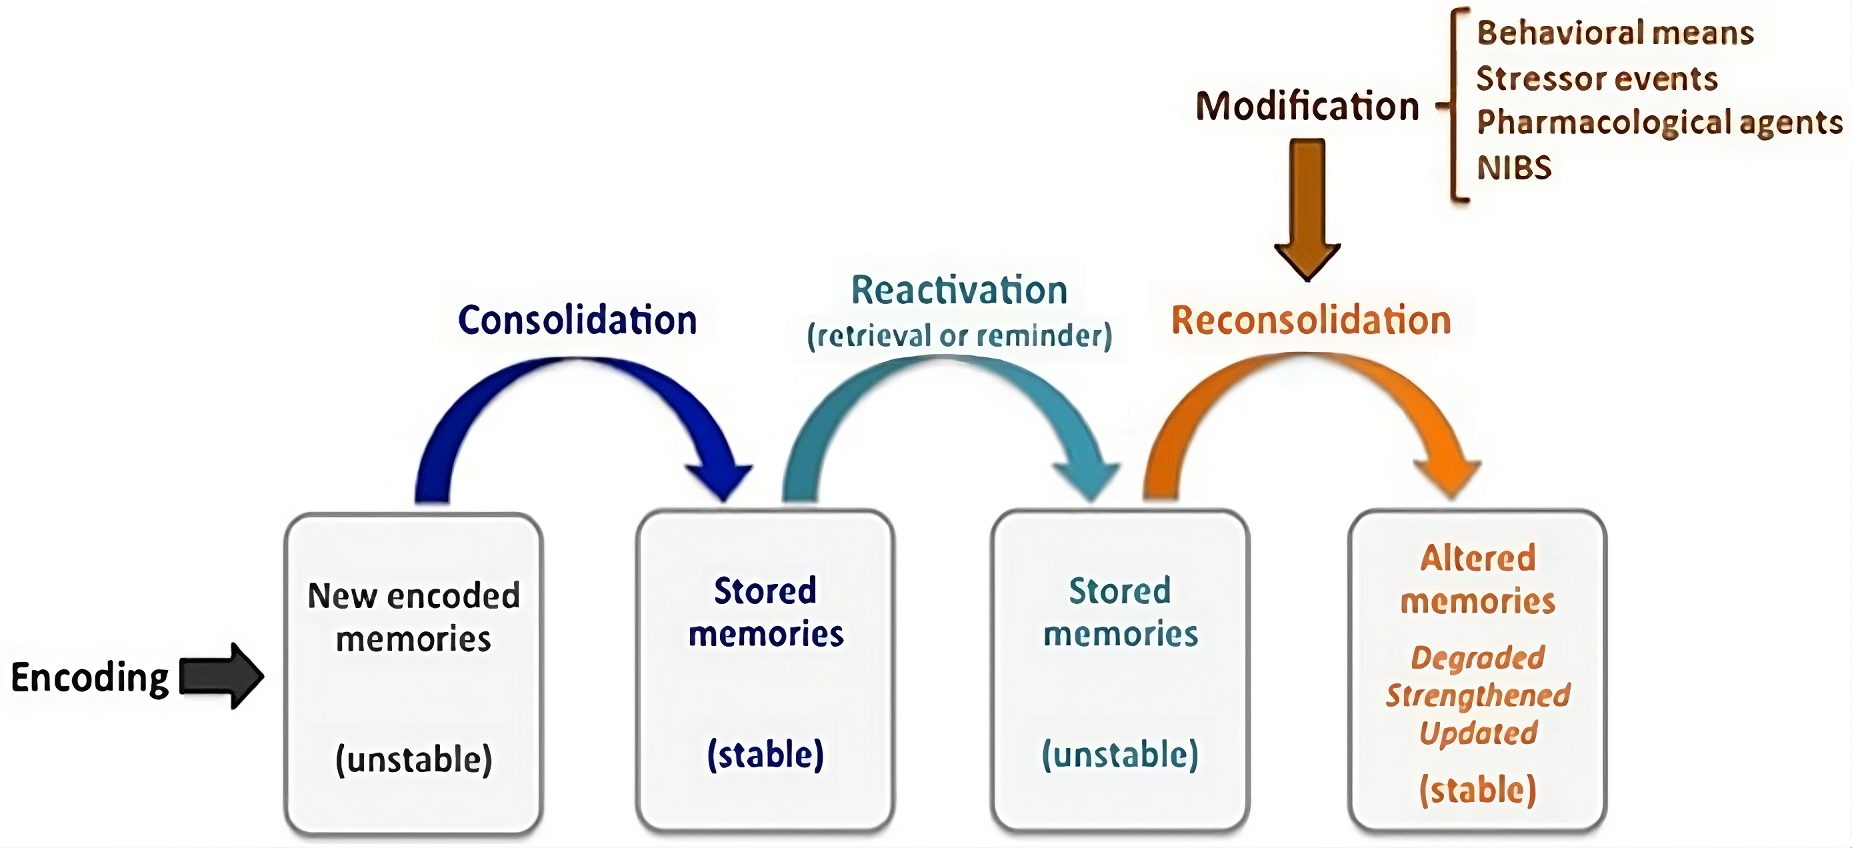
\includegraphics[width=0.6\linewidth]{./img/memory.png}
    \caption{Memory flow}
\end{figure}

\begin{remark}
    This mechanism is useful against traumatic memories.
\end{remark}

\begin{remark}
    The amygdala is responsible for storing conditioned responses while the hippocampus recognizes conditioned stimuli.

    Patients with a damaged amygdala only recognize \ac{cs} but do not act with any \ac{cr}.
    On the other hand, a damaged hippocampus results in patients that present a \ac{cr} without recognizing the \ac{cs}.
\end{remark}

\begin{casestudy}[Reconsolidation disruption]
    Propranolol is a drug that disrupts amygdala-specific memory reconsolidation (i.e. the physiological response).
    A possible therapy to suppress a phobia is to trigger the fear memory and then administer propranolol to prevent its reconsolidation.
\end{casestudy}



\section{Learning preconditions}

\subsection{Contiguity}
\marginnote{Contiguity}

Closeness between the \acl{cs} and the \acl{us}.

\begin{remark}
    The closer in time the stimuli are presented, the more likely the association will be created.
\end{remark}

Depending on when the \ac{cs} and \ac{us} are presented, conditioning can be:
\begin{descriptionlist}
    \item[Delay conditioning] \marginnote{Delay conditioning}
        The \ac{cs} is extended through the interstimulus interval (ISI) (i.e. time between the start of the \ac{cs} and the \ac{us}).

    \item[Trace conditioning] \marginnote{Trace conditioning}
        There is a delay (trace interval) between the \ac{cs} end and the \ac{us} start.

        Learning requires more trials and might be impossible if the trace interval is too long as the mental representation of the \ac{cs} decays.

    \begin{figure}[H]
        \centering
        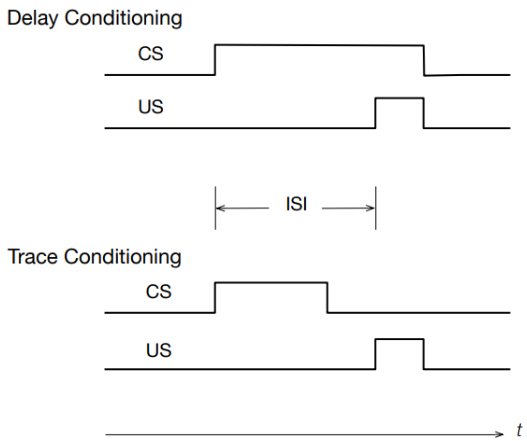
\includegraphics[width=0.45\linewidth]{./img/contiguity.png}
    \end{figure}
\end{descriptionlist}

\begin{casestudy}
    Two groups of rats were exposed to a 6 seconds tone (\ac{cs}) followed by food delivery (\ac{us}) with a delay of: 
    \begin{itemize}
        \item 6 seconds (red).
        \item 18 seconds (purple).
    \end{itemize}

    \begin{figure}[H]
        \centering
        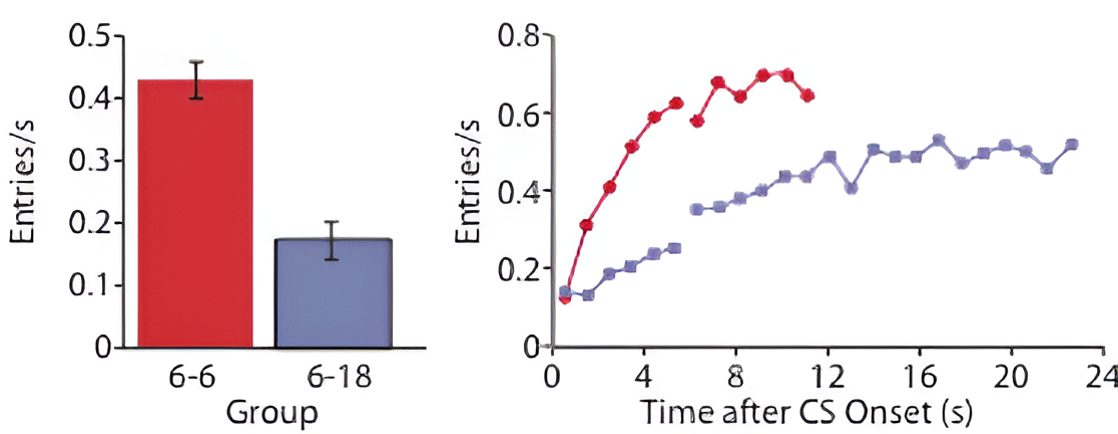
\includegraphics[width=0.55\linewidth]{./img/contiguity_rats.png}
        \caption{Number of entries (i.e. the rat checks the food tray) per second}
    \end{figure}
\end{casestudy}


\subsection{Contingency}
\marginnote{Contingency}

Causal relationship between the \acl{cs} and the \acl{us}.

\begin{remark}
    Learning happens when:
    \[ \prob{\text{\ac{us} with \ac{cs}}} > \prob{\text{\ac{us} with no \ac{cs}}} \]
    In other words, the \ac{cs} should provide information regarding the \ac{us}.
\end{remark}

\begin{figure}[H]
    \centering
    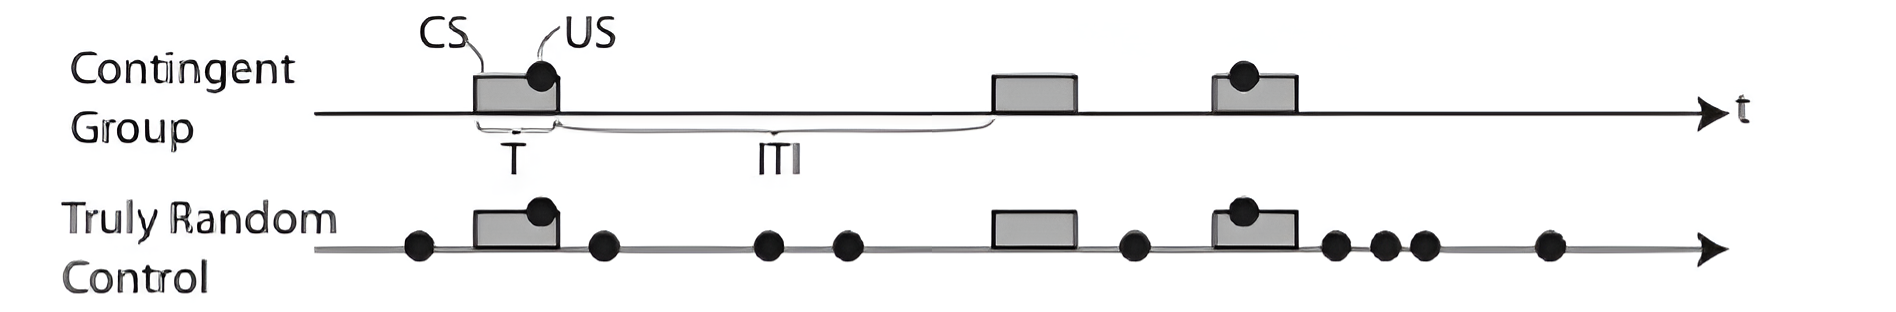
\includegraphics[width=0.6\linewidth]{./img/contingency.png}
    \caption{Example of contingent and random group}
\end{figure}

\begin{casestudy}
    Two groups of rats are exposed to a shock paired with a bell ring.
    Contiguity is the same but contingency differs.

    Only the group where the shock is more likely with the bell learns the association.

    \begin{figure}[H]
        \centering
        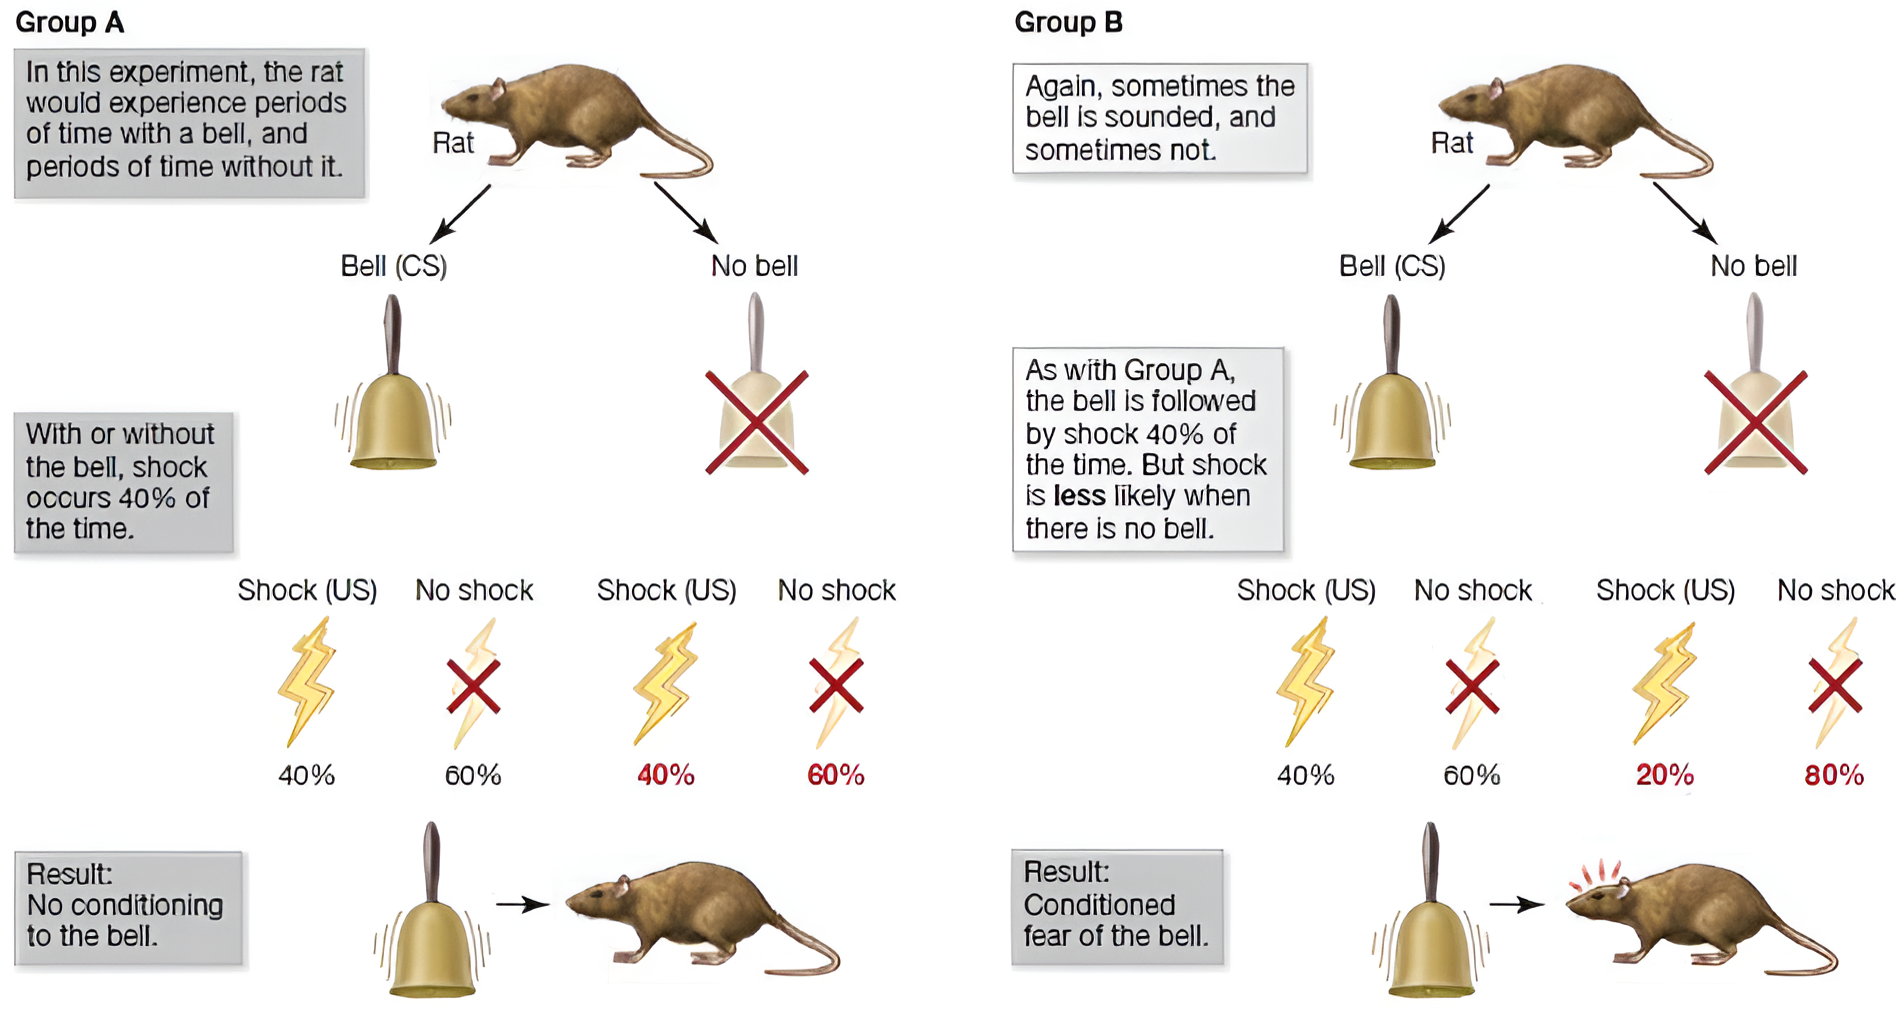
\includegraphics[width=0.8\linewidth]{./img/contingency_rats.png}
        \caption{Representation of the experiment}
    \end{figure}
\end{casestudy}


\subsection{Surprise}

\begin{description}
    \item[Prediction error] \marginnote{Prediction error}
        Quantitative discrepancy between the expected and experienced outcome.
\end{description}

\begin{remark}
    Learning happens when the outcome is different from what was expected.
\end{remark}

\begin{figure}[H]
    \centering
    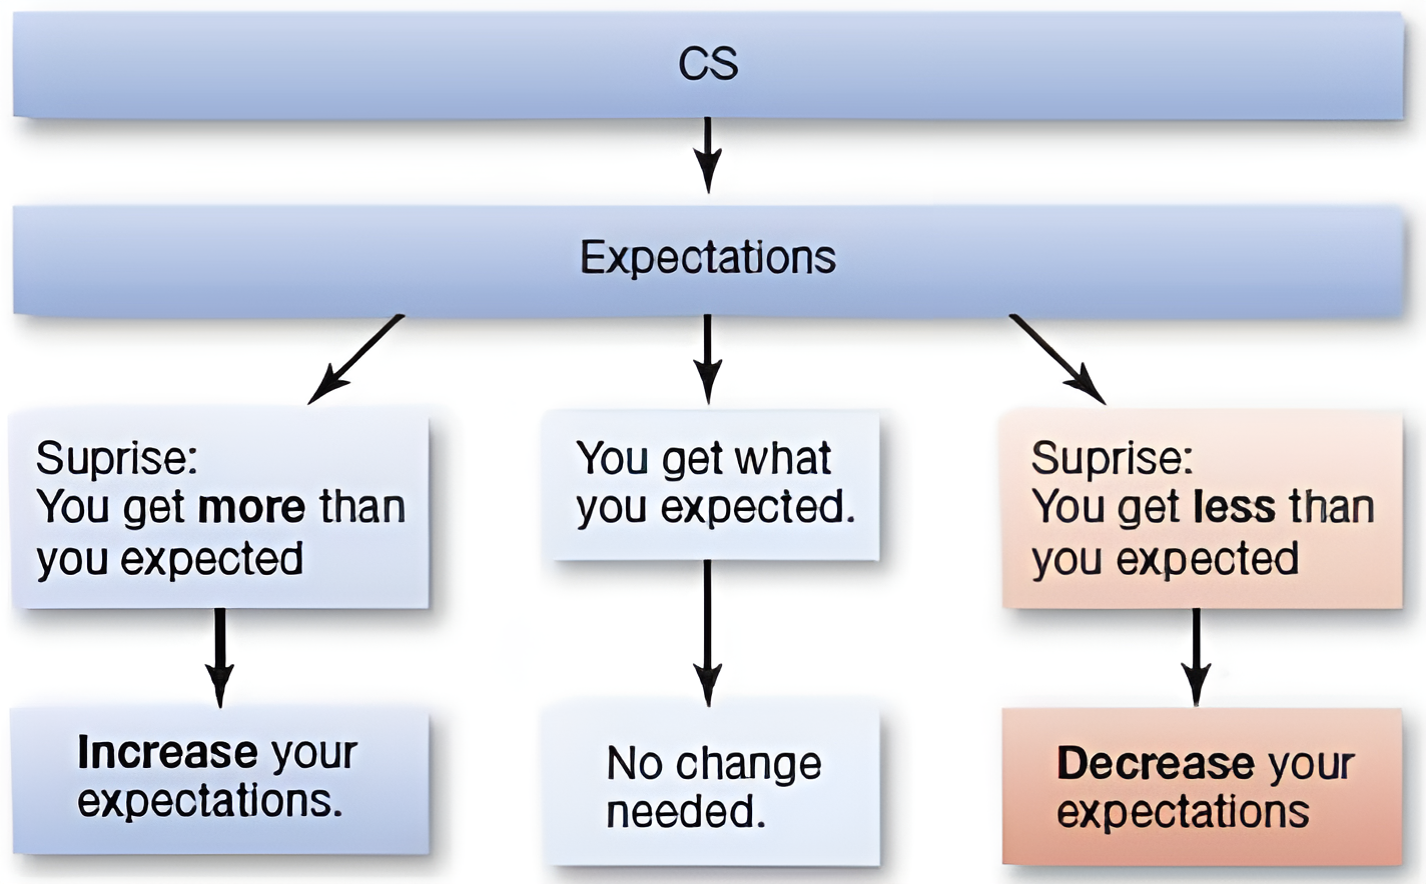
\includegraphics[width=0.4\linewidth]{./img/surprise.png}
    \caption{Learning outcome due to surprise}
\end{figure}

\begin{casestudy}[Blocking effect]
    \phantom{} \label{ex:blocking} \\
    \begin{minipage}{0.65\linewidth}
        \begin{enumerate}
            \item A rat is taught that a hissing sound (\ac{cs}) is paired with a sexually receptive mate (\ac{us}).
            \item A light is added together with the hissing sound.
            \item When only the light is presented, the rat does not provide a response.
        \end{enumerate}

        The light is not learned as a \ac{cs} as it does not provide any new information on the \ac{us}.
    \end{minipage}
    \begin{minipage}{0.35\linewidth}
        \begin{figure}[H]
            \centering
            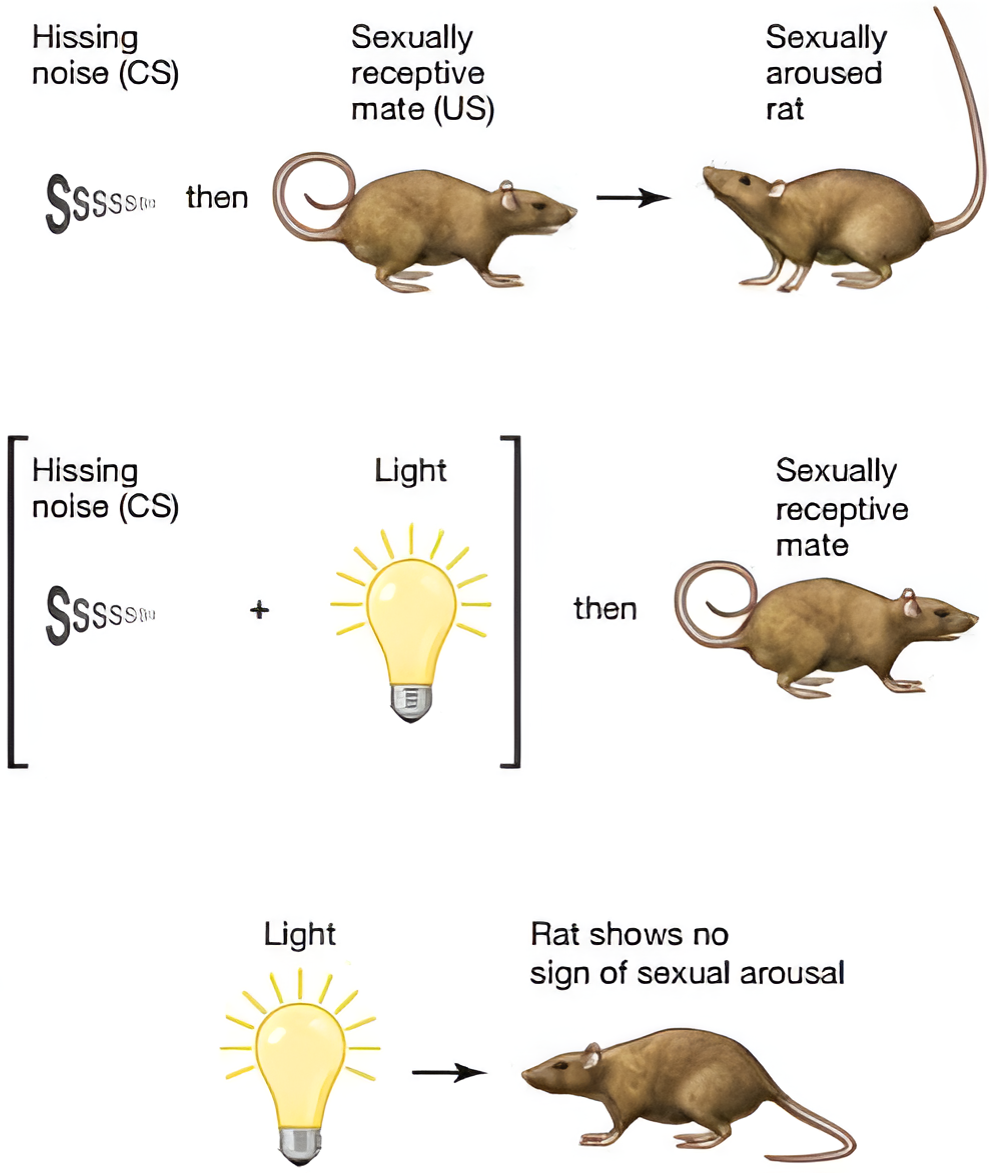
\includegraphics[width=\linewidth]{./img/surprise_rats.png}
        \end{figure}
    \end{minipage}
\end{casestudy}



\section{Computational model}


\subsection{Rescorla-Wagner model}
\marginnote{Rescorla-Wagner model}

Error-driven learning model where the change expectancy is proportional to the difference between predicted and actual outcome:
\[ \delta_{tr} = R_{tr} - V_{tr} \]
where:
\begin{itemize}
    \item $\delta_{tr}$ is the prediction error.
    \item $R_{tr} = \begin{cases}
            1 & \text{if the \ac{us} is delivered at trial $tr$} \\
            0 & \text{if the \ac{us} is omitted at trial $tr$}
        \end{cases}$.
    \item $V_{tr}$ is the association strength (i.e. expectancy of the \ac{us} or the expected value resulting from a given \ac{cs}) at trial $tr$.
\end{itemize}

Then, the expected value $V_{tr+1}$ is obtained as:
\[ V_{tr+1} = V_{tr} + \alpha \delta_{tr} \]
where $\alpha \in [0, 1]$ is the learning rate.

\begin{remark}
    A lower $\alpha$ is more suited for volatile environments.
\end{remark}

\begin{remark}
    The prediction error $\delta$ is:
    \begin{itemize}
        \item Positive during acquisition.
        \item Negative during extinction.
    \end{itemize}
    Moreover, the error is larger at the start of acquisition/extinction.
\end{remark}

\begin{remark}
    The Rescorla-Wagner model is able to capture the blocking effect (see \hyperref[ex:blocking]{Blocking example}) as
    the animal computes a single prediction error obtained as the combination of multiple stimuli.
\end{remark}

\begin{figure}[H]
    \centering
    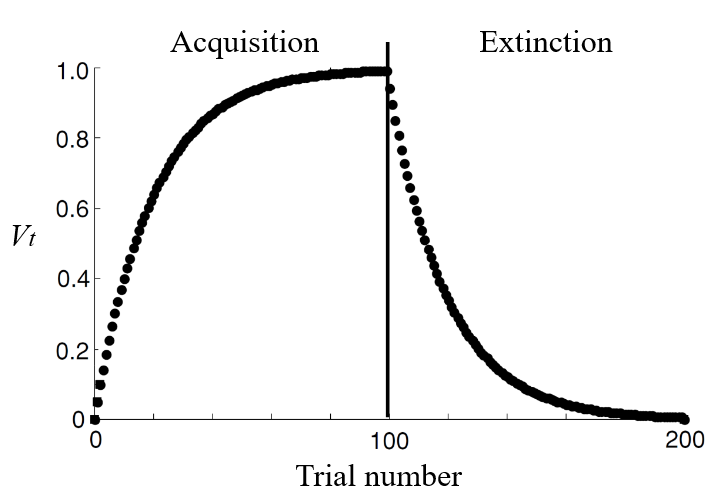
\includegraphics[width=0.4\linewidth]{./img/rescorla_wagner_curve.png}
    \caption{Acquisition and extinction in Pavlovian learning according to the Rescorla-Wagner model}
\end{figure}

\begin{remark}
    The Rescorla-Wagner model is a trial-level model that only considers the change from trial to trial
    without considering what happens within and between trials.
\end{remark}


\subsection{Temporal difference model}
\marginnote{Temporal difference model}

Real-time model based on time steps within a trial instead of monolithic trials.
At each time $t$ of a trial during which a \ac{cs} is presented,
the model computes a prediction of the total future reward that will be gained from time $t$ to the end of the trial.

The prediction error is computed as follows\footnote{\url{https://pubmed.ncbi.nlm.nih.gov/9054347/}}:
\begin{gather*}
    \delta_t = R_t + V_{t+1} - V_t \\
    V_{t+1} = V_t + \alpha \delta_t
\end{gather*}

\begin{itemize}
    \item At the beginning of learning, the \ac{cs} is presented at time $t_\text{\ac{cs}}$
        and $V_t = 0$ until the \ac{us} is delivered at time $t_\text{\ac{us}} > t_\text{\ac{cs}}$.
    \item On the next trial, $V_{t_\text{\ac{us}}} - V_{t_\text{\ac{us}} - 1}$ now generates a positive prediction error that updates $V_{t_\text{\ac{us}} - 1}$.
    \item On subsequent trials, $V_t$ is updated for each $t$ in between $t_\text{\ac{us}}$ back to $t_\text{\ac{cs}}$.
\end{itemize}

In other words, the value signal produced by the reward (\ac{us}) is transferred back to an event (\ac{cs}) that predicts the reward.

\begin{casestudy}[Second-order conditioning]
    Pairing a new \ac{cs} to an existing \ac{cs}.

    \begin{center}
        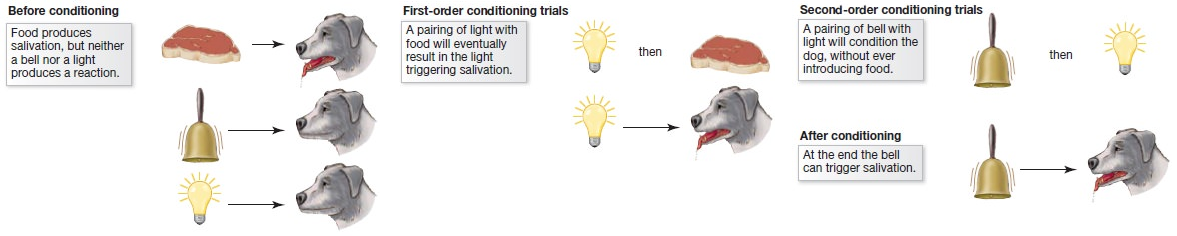
\includegraphics[width=0.95\linewidth]{./img/second_order_conditioning.png}
    \end{center}

    \begin{remark}
        The Rescorla-Wagner model is not capable of modeling second-order conditioning while 
        the temporal difference model is.
    \end{remark}
\end{casestudy}



\section{Reward prediction error hypothesis of dopamine}

There is strong evidence that the dopaminergic system is the major neural mechanism of reward and reinforcement.

\begin{description}
    \item[Response to unexpected rewards] \marginnote{Dopamine response to unexpected rewards}
        Dopaminergic neurons exhibit a strong phasic response in the presence of an unexpected reward.

        \begin{casestudy}[Monkey that touches food]
            Some food is put in a box with a hole to reach its content.
            In the absence of any other stimuli predicting the reward, 
            a monkey presents a high dopaminergic response when it touches the food.
            \begin{center}
                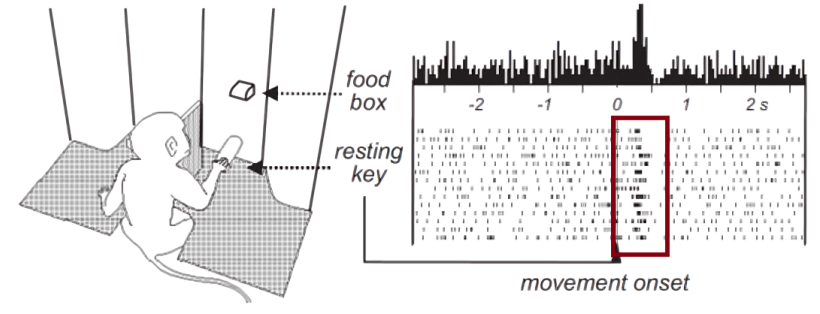
\includegraphics[width=0.55\linewidth]{./img/dopamine_monkey1.png}    
            \end{center}
        \end{casestudy}

    \item[Reward discrimination] \marginnote{Dopamine reward discrimination}
        Dopamine neurons respond differently depending on the actual presence of a reward.

        \begin{casestudy}[Monkey that touches food]
            The dopaminergic response of a monkey that touches an apple attached to a wire in a box is different 
            from the response of only touching the wire.
            \begin{center}
                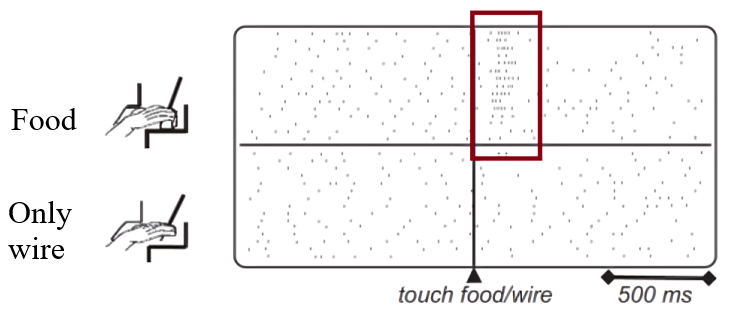
\includegraphics[width=0.5\linewidth]{./img/dopamine_monkey2.png}    
            \end{center}
        \end{casestudy}

    \item[Magnitude discrimination] \marginnote{Dopamine magnitude discrimination}
        Dopamine neurons respond differently depending on the amount of reward received.

        \begin{casestudy}[Monkey that drinks]
            By giving a monkey different amounts of fruit juice in a pseudorandom order,
            its dopaminergic response is stronger for the highest volume and weaker for the lowest volume.
            \begin{center}
                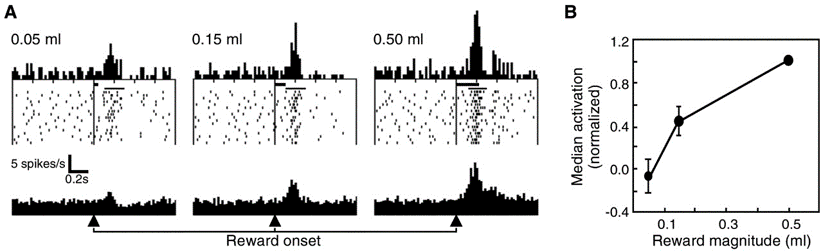
\includegraphics[width=0.7\linewidth]{./img/dopamine_monkey3.png}    
            \end{center}
        \end{casestudy}

        \begin{casestudy}[Monkey with juice and images]
            Using different \acp{cs}, it can be seen that the dopaminergic response differs based on the amount of reward.
            \begin{center}
                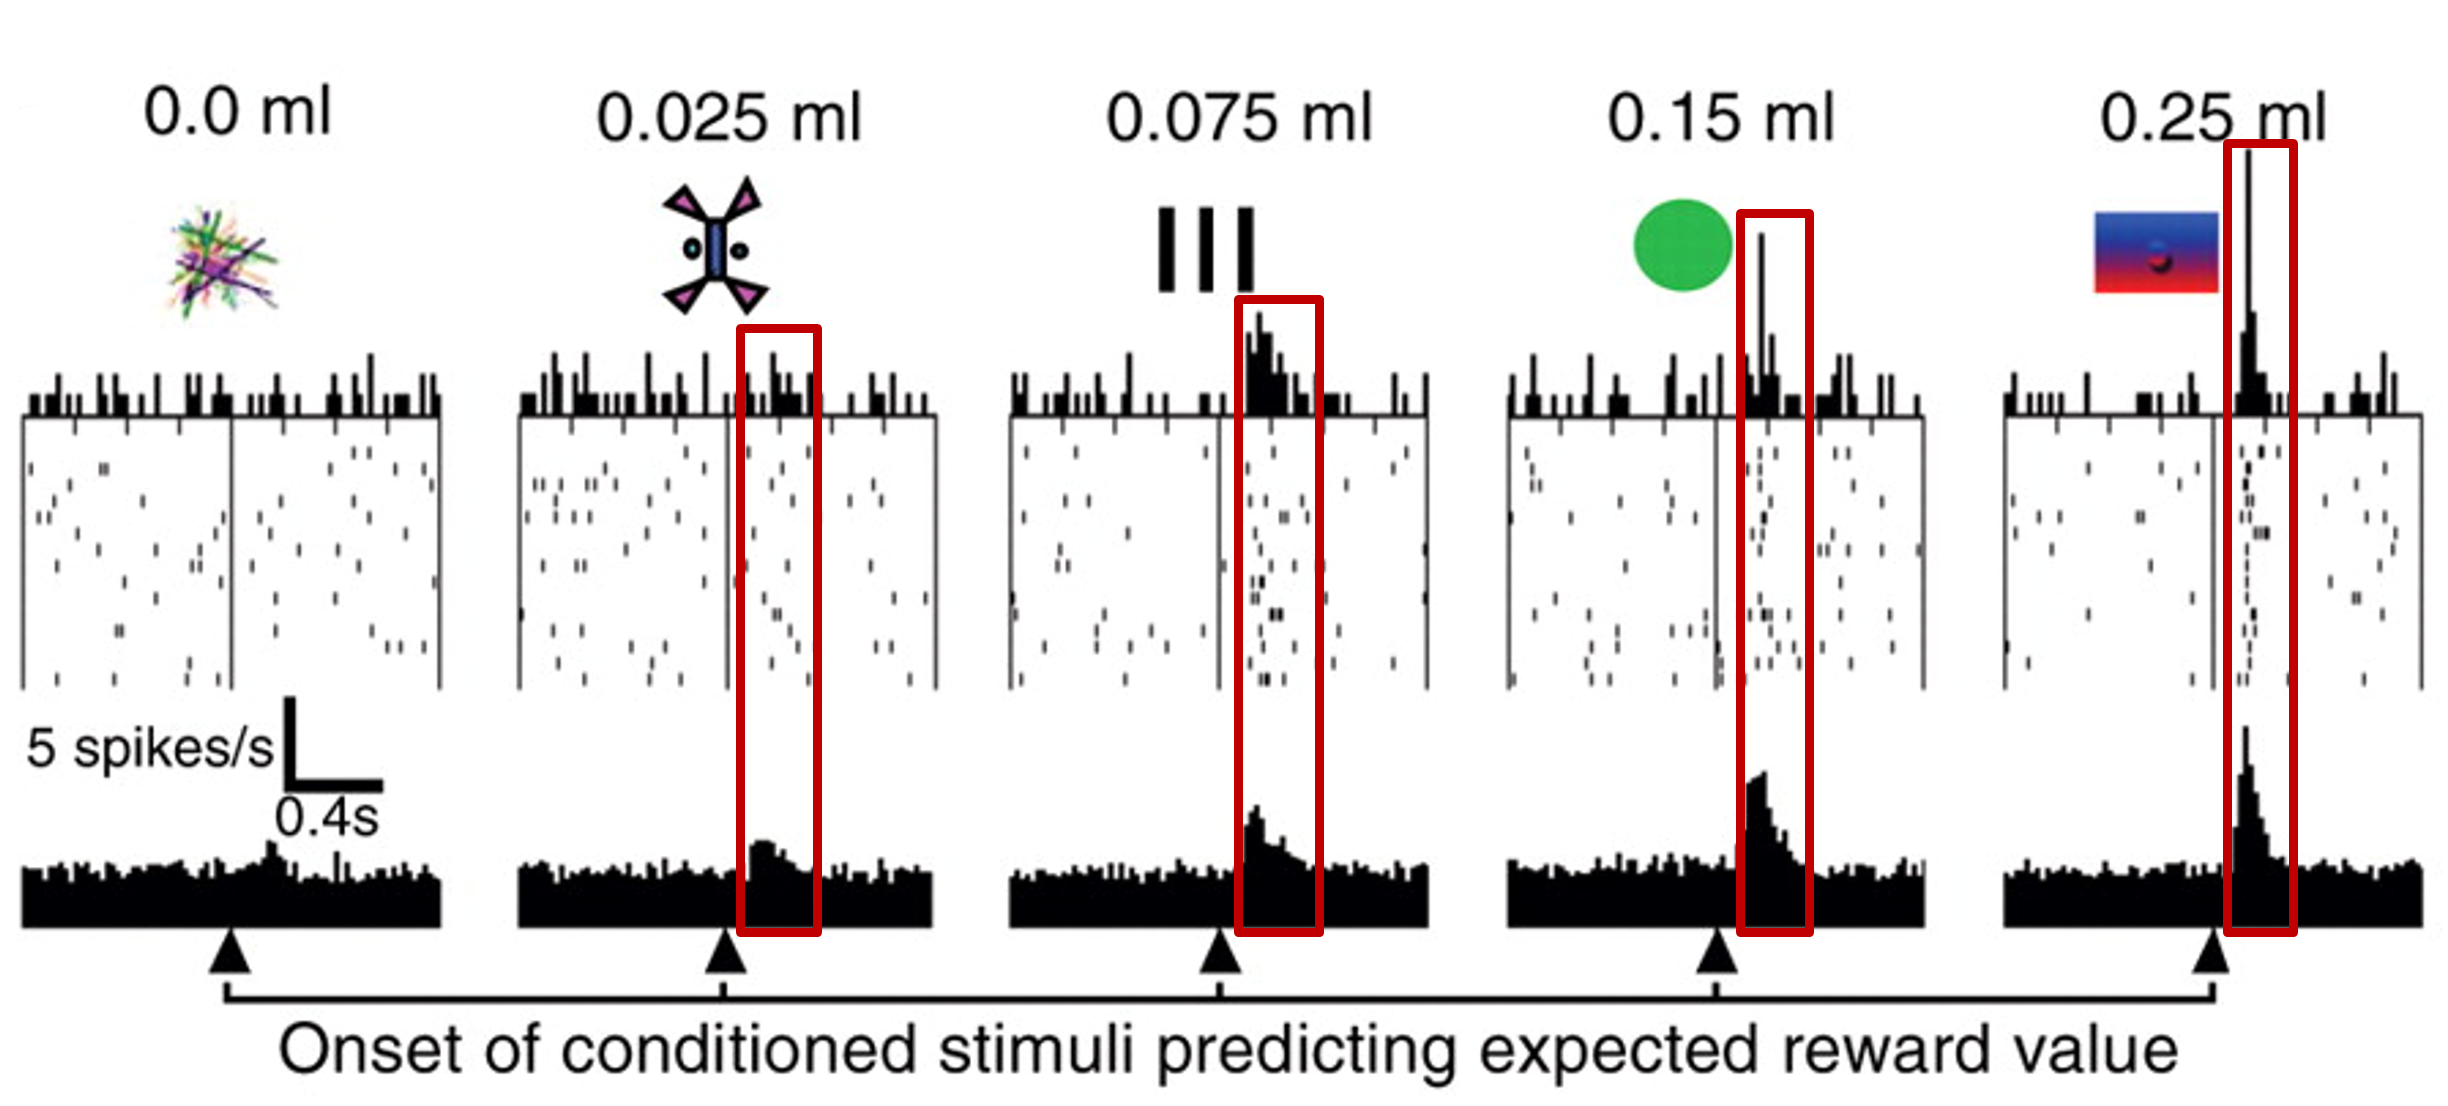
\includegraphics[width=0.55\linewidth]{./img/dopamine_expected.png}
            \end{center}
        \end{casestudy}

        \begin{casestudy}[Monkey with juice and images]
            After learning the association between a \ac{cs} and \ac{us} (middle graph), a change in the amount of the reward changes the dopaminergic response.
            \begin{center}
                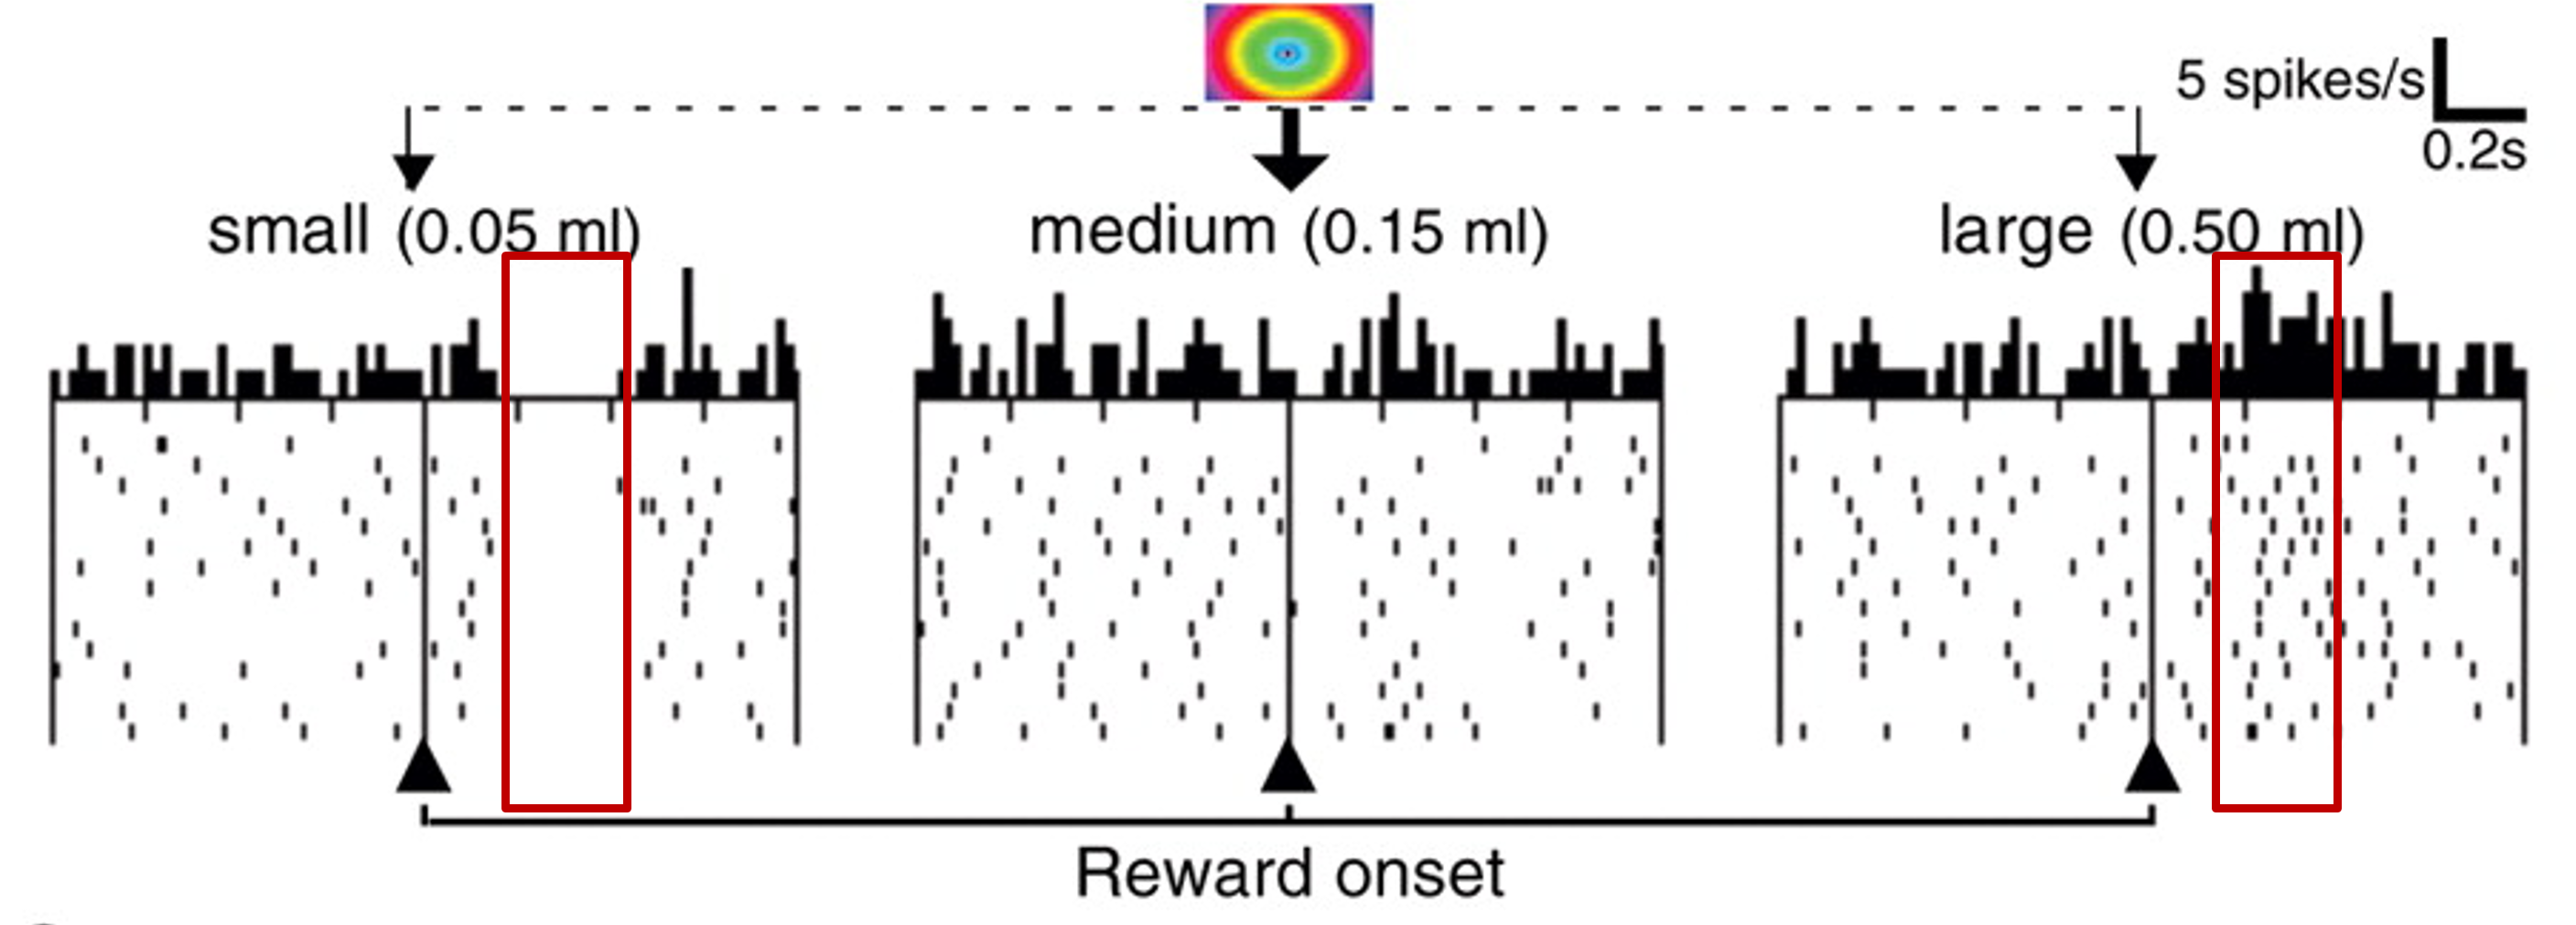
\includegraphics[width=0.6\linewidth]{./img/dopamine_expected2.png}
            \end{center}

            This behavior also involves the context (i.e. the \ac{cs} image that is shown).
            \begin{center}
                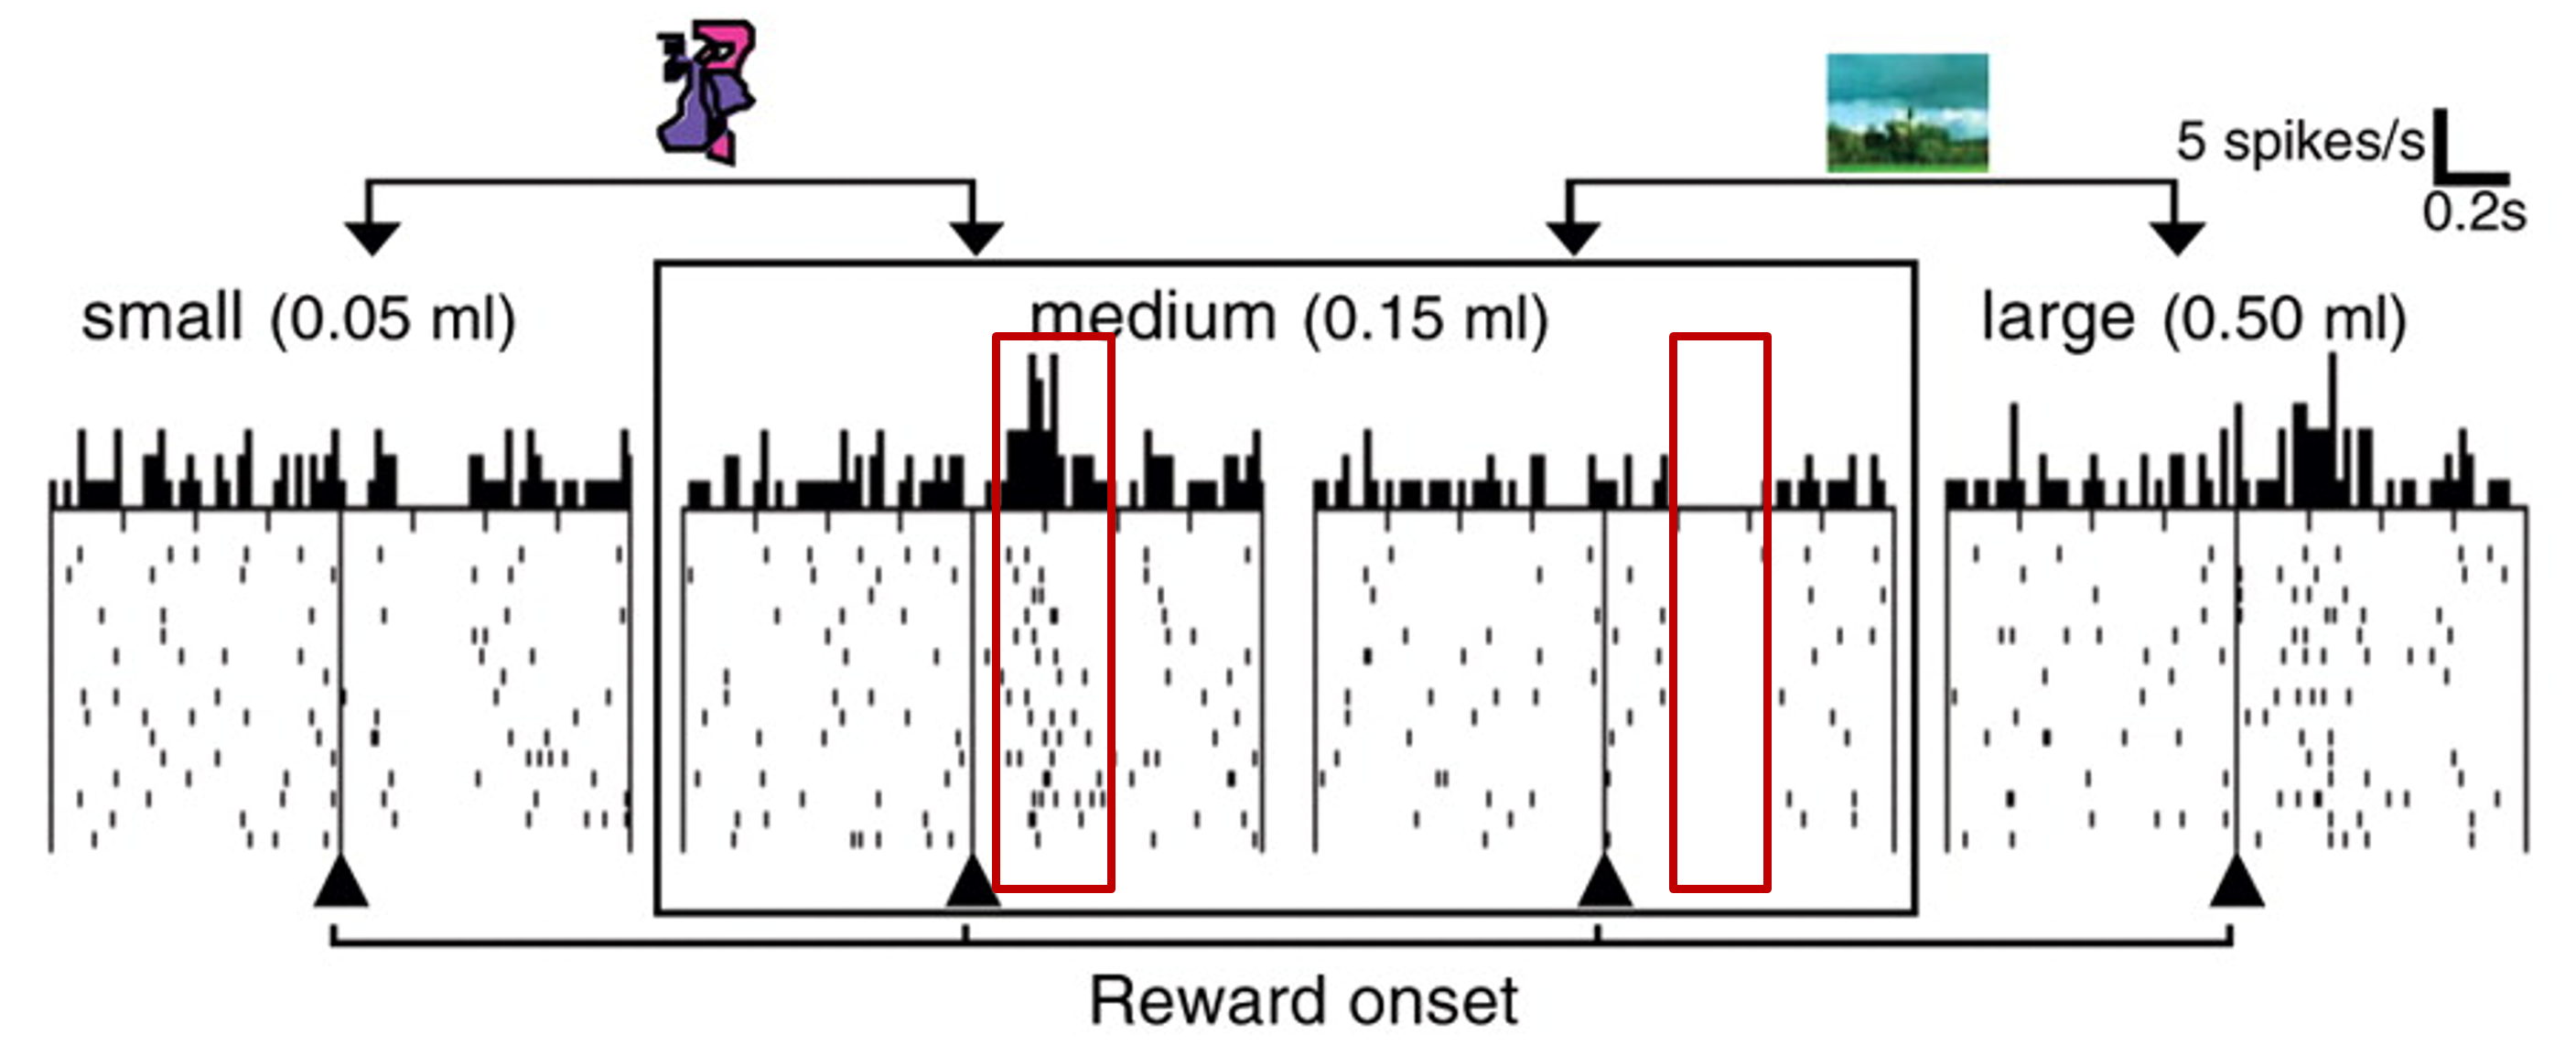
\includegraphics[width=0.6\linewidth]{./img/dopamine_expected3.png}
            \end{center}
        \end{casestudy}
\end{description}

\begin{remark}
    With the previous observations, it can be concluded that:
    \begin{itemize}
        \item Dopamine neurons increase their firing rate when the reward is unexpectedly delivered or better than expected.
        \item Dopamine neurons decrease their firing rate when the reward is unexpectedly omitted or worse than expected.
    \end{itemize}
\end{remark}

\begin{description}
    \item[Transfer to \ac{cs}] \marginnote{Dopamine transfer to \ac{cs}}
        \begin{itemize}
            \item Before training, an unexpected reward (\ac{us}) causes the dopamine neurons to increase firing (positive prediction error).
            \item After training, dopamine neurons firing is increased after the \ac{cs} but not following the reward (no prediction error).
            \item After training, dopamine neurons firing is increased after the \ac{cs} but is decreased if the reward is omitted (negative prediction error).
        \end{itemize}
        \begin{center}
            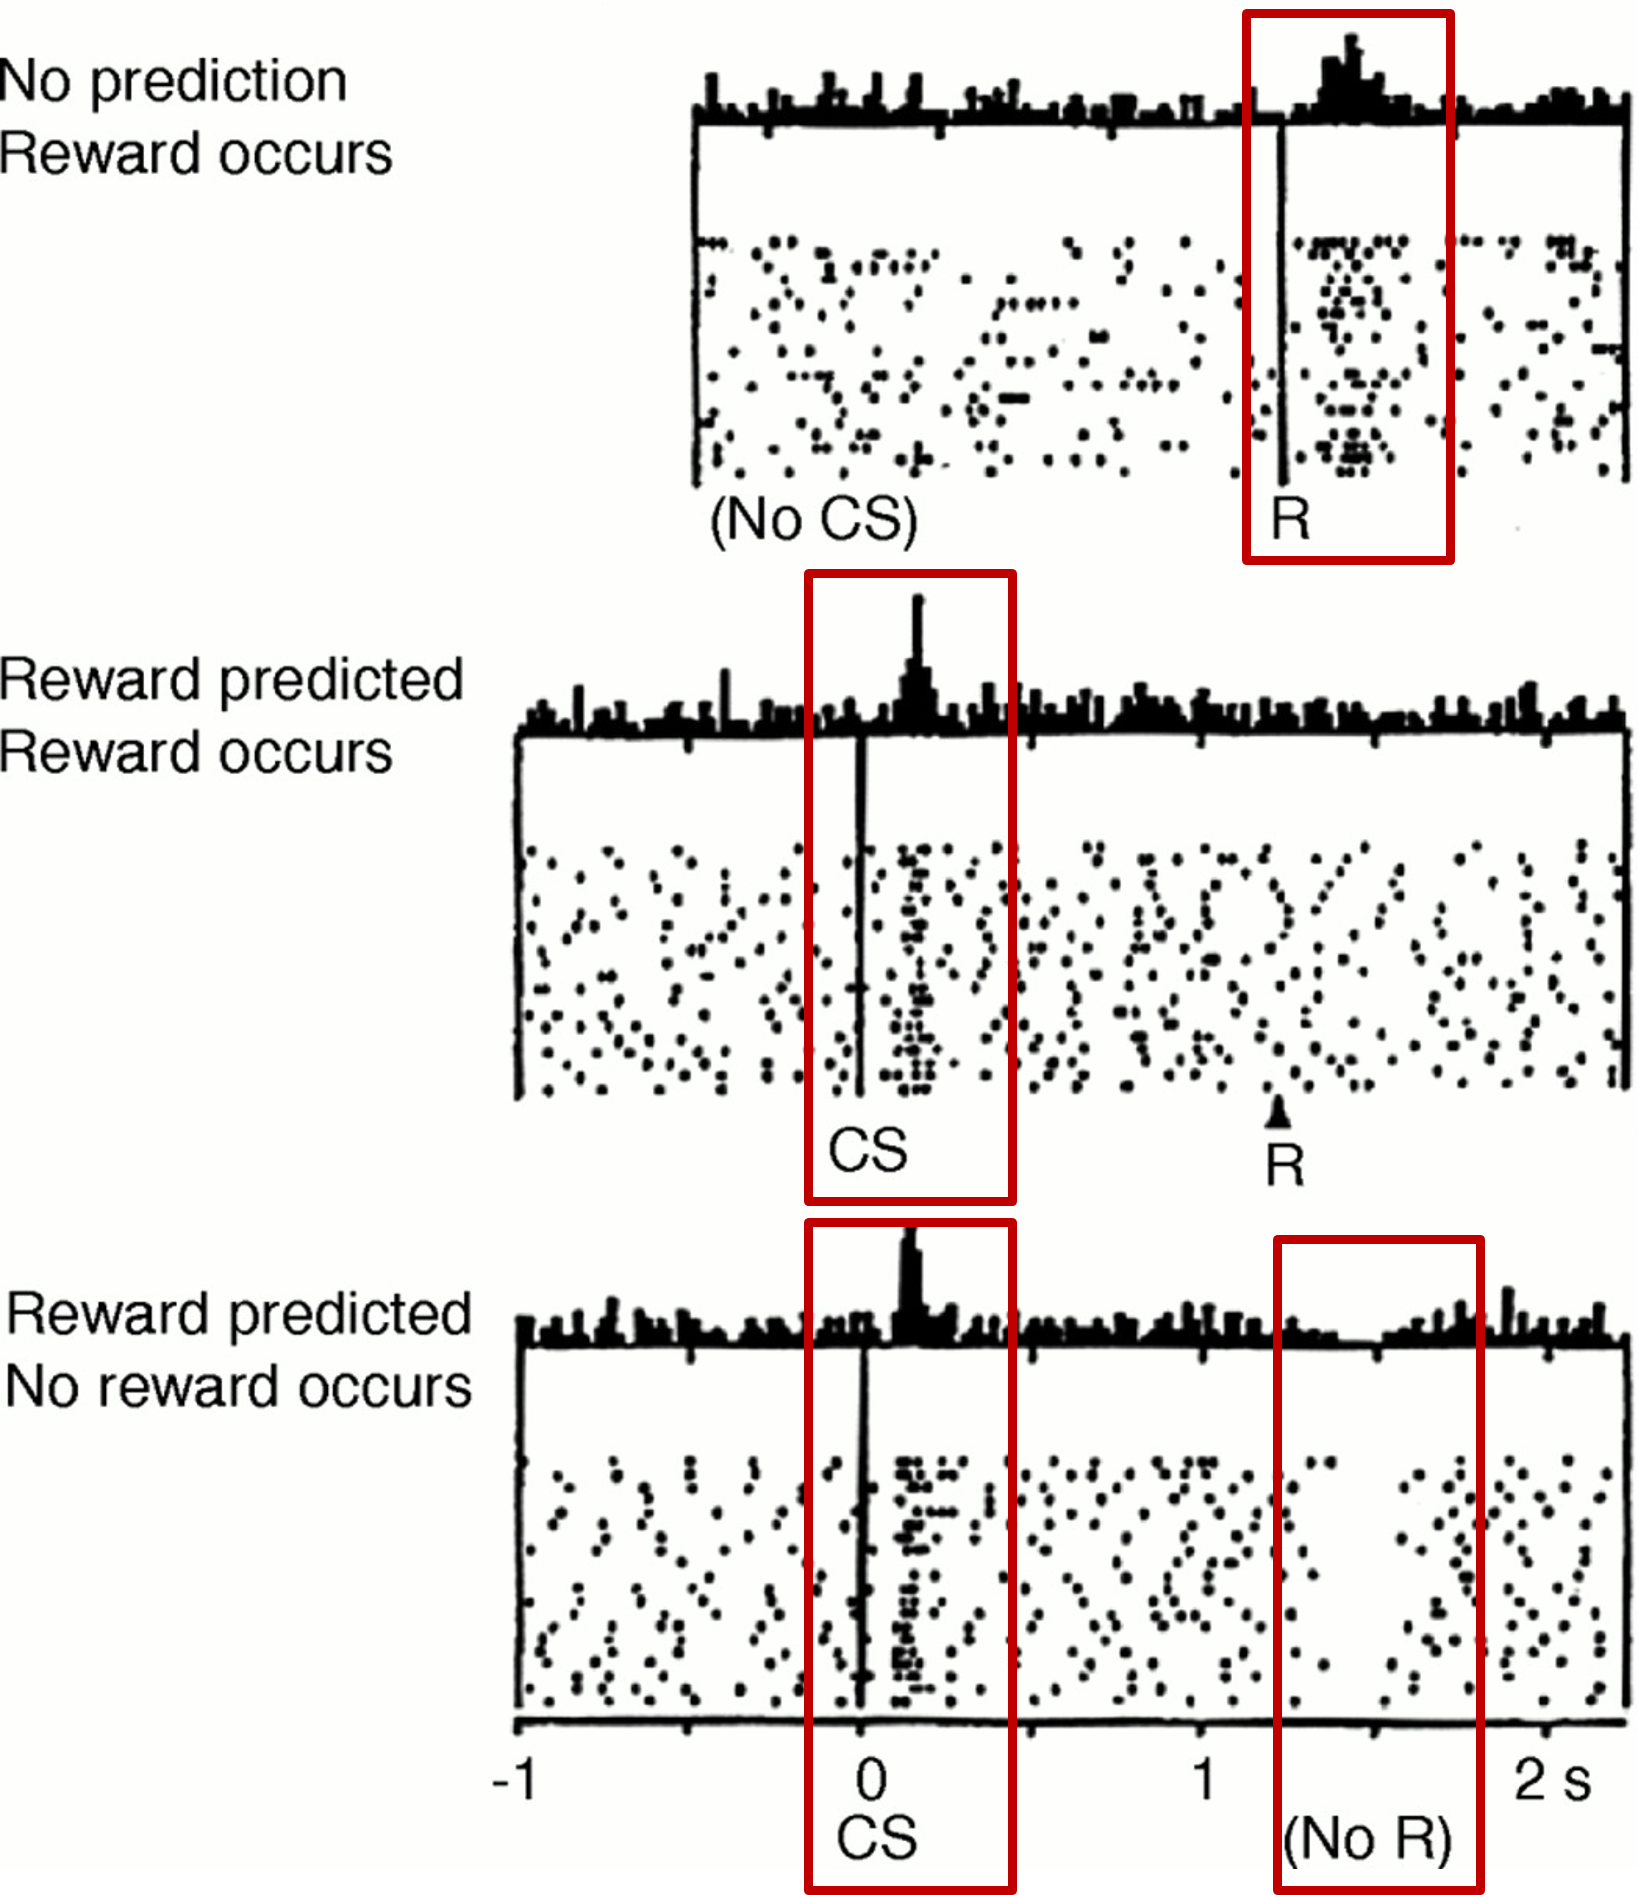
\includegraphics[width=0.4\linewidth]{./img/dopamine_transfer_cs.png}
        \end{center}

    \item[Response to blocking] \marginnote{Dopamine response to blocking}
        Dopaminergic response is in line with the blocking effect.

        \begin{casestudy}[Monkey with food and images]
            \phantom{}\\
            \begin{minipage}{0.7\linewidth}
                A monkey is taught to associate images with food.
                A new \ac{cs} alongside an existing \ac{cs} will not be learned.
            \end{minipage}
            \begin{minipage}{0.28\linewidth}
                \centering
                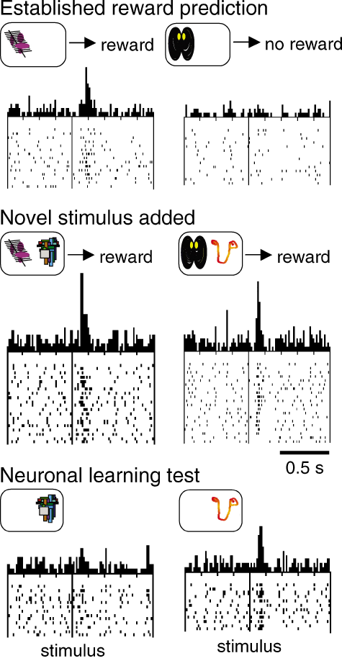
\includegraphics[width=\linewidth]{./img/dopamine_blocking.png}
            \end{minipage}
        \end{casestudy}

    \item[Probability encoding] \marginnote{Dopamine probability encoding}
        The phasic activation of dopamine neurons varies monotonically with the reward probability
        \begin{center}
            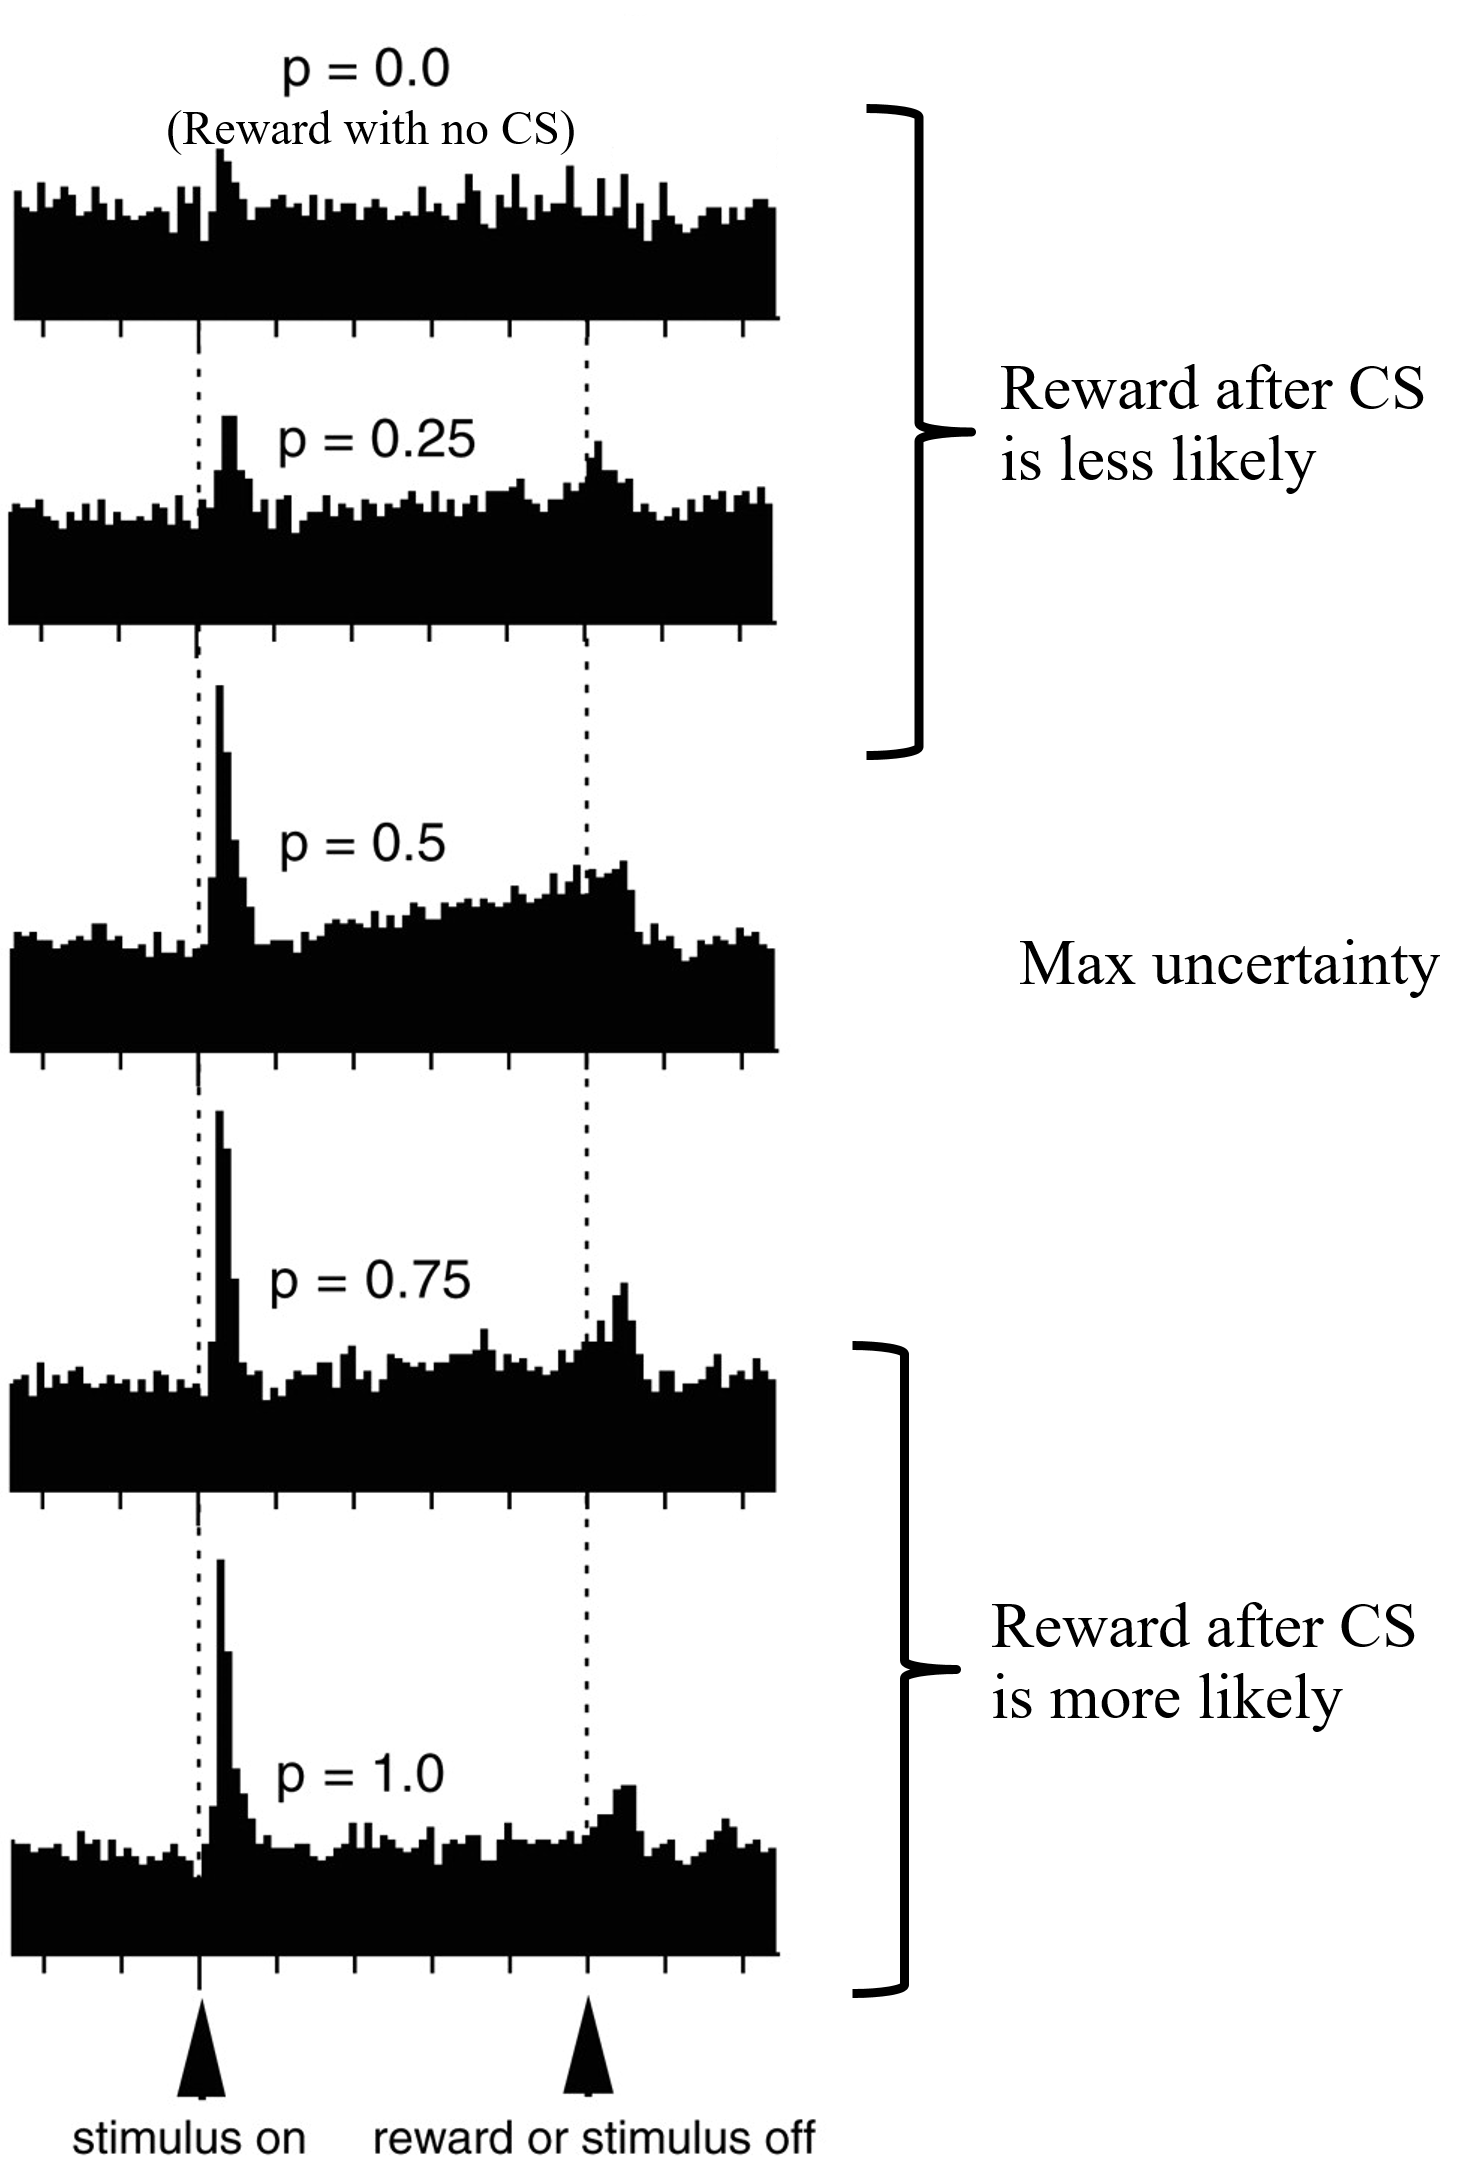
\includegraphics[width=0.65\linewidth]{./img/dopamine_probability.png}
        \end{center}

    \item[Timing encoding] \marginnote{Dopamine timing encoding}
        Dopamine response to unexpectedness also involves timing.
        A dopaminergic response occurs when a reward is given earlier or later than expected.

        \begin{casestudy}
            After learning that a reward occurs 1 second after the end of the \ac{cs}, 
            dopamine neurons fire if the timing changes.
            \begin{center}
                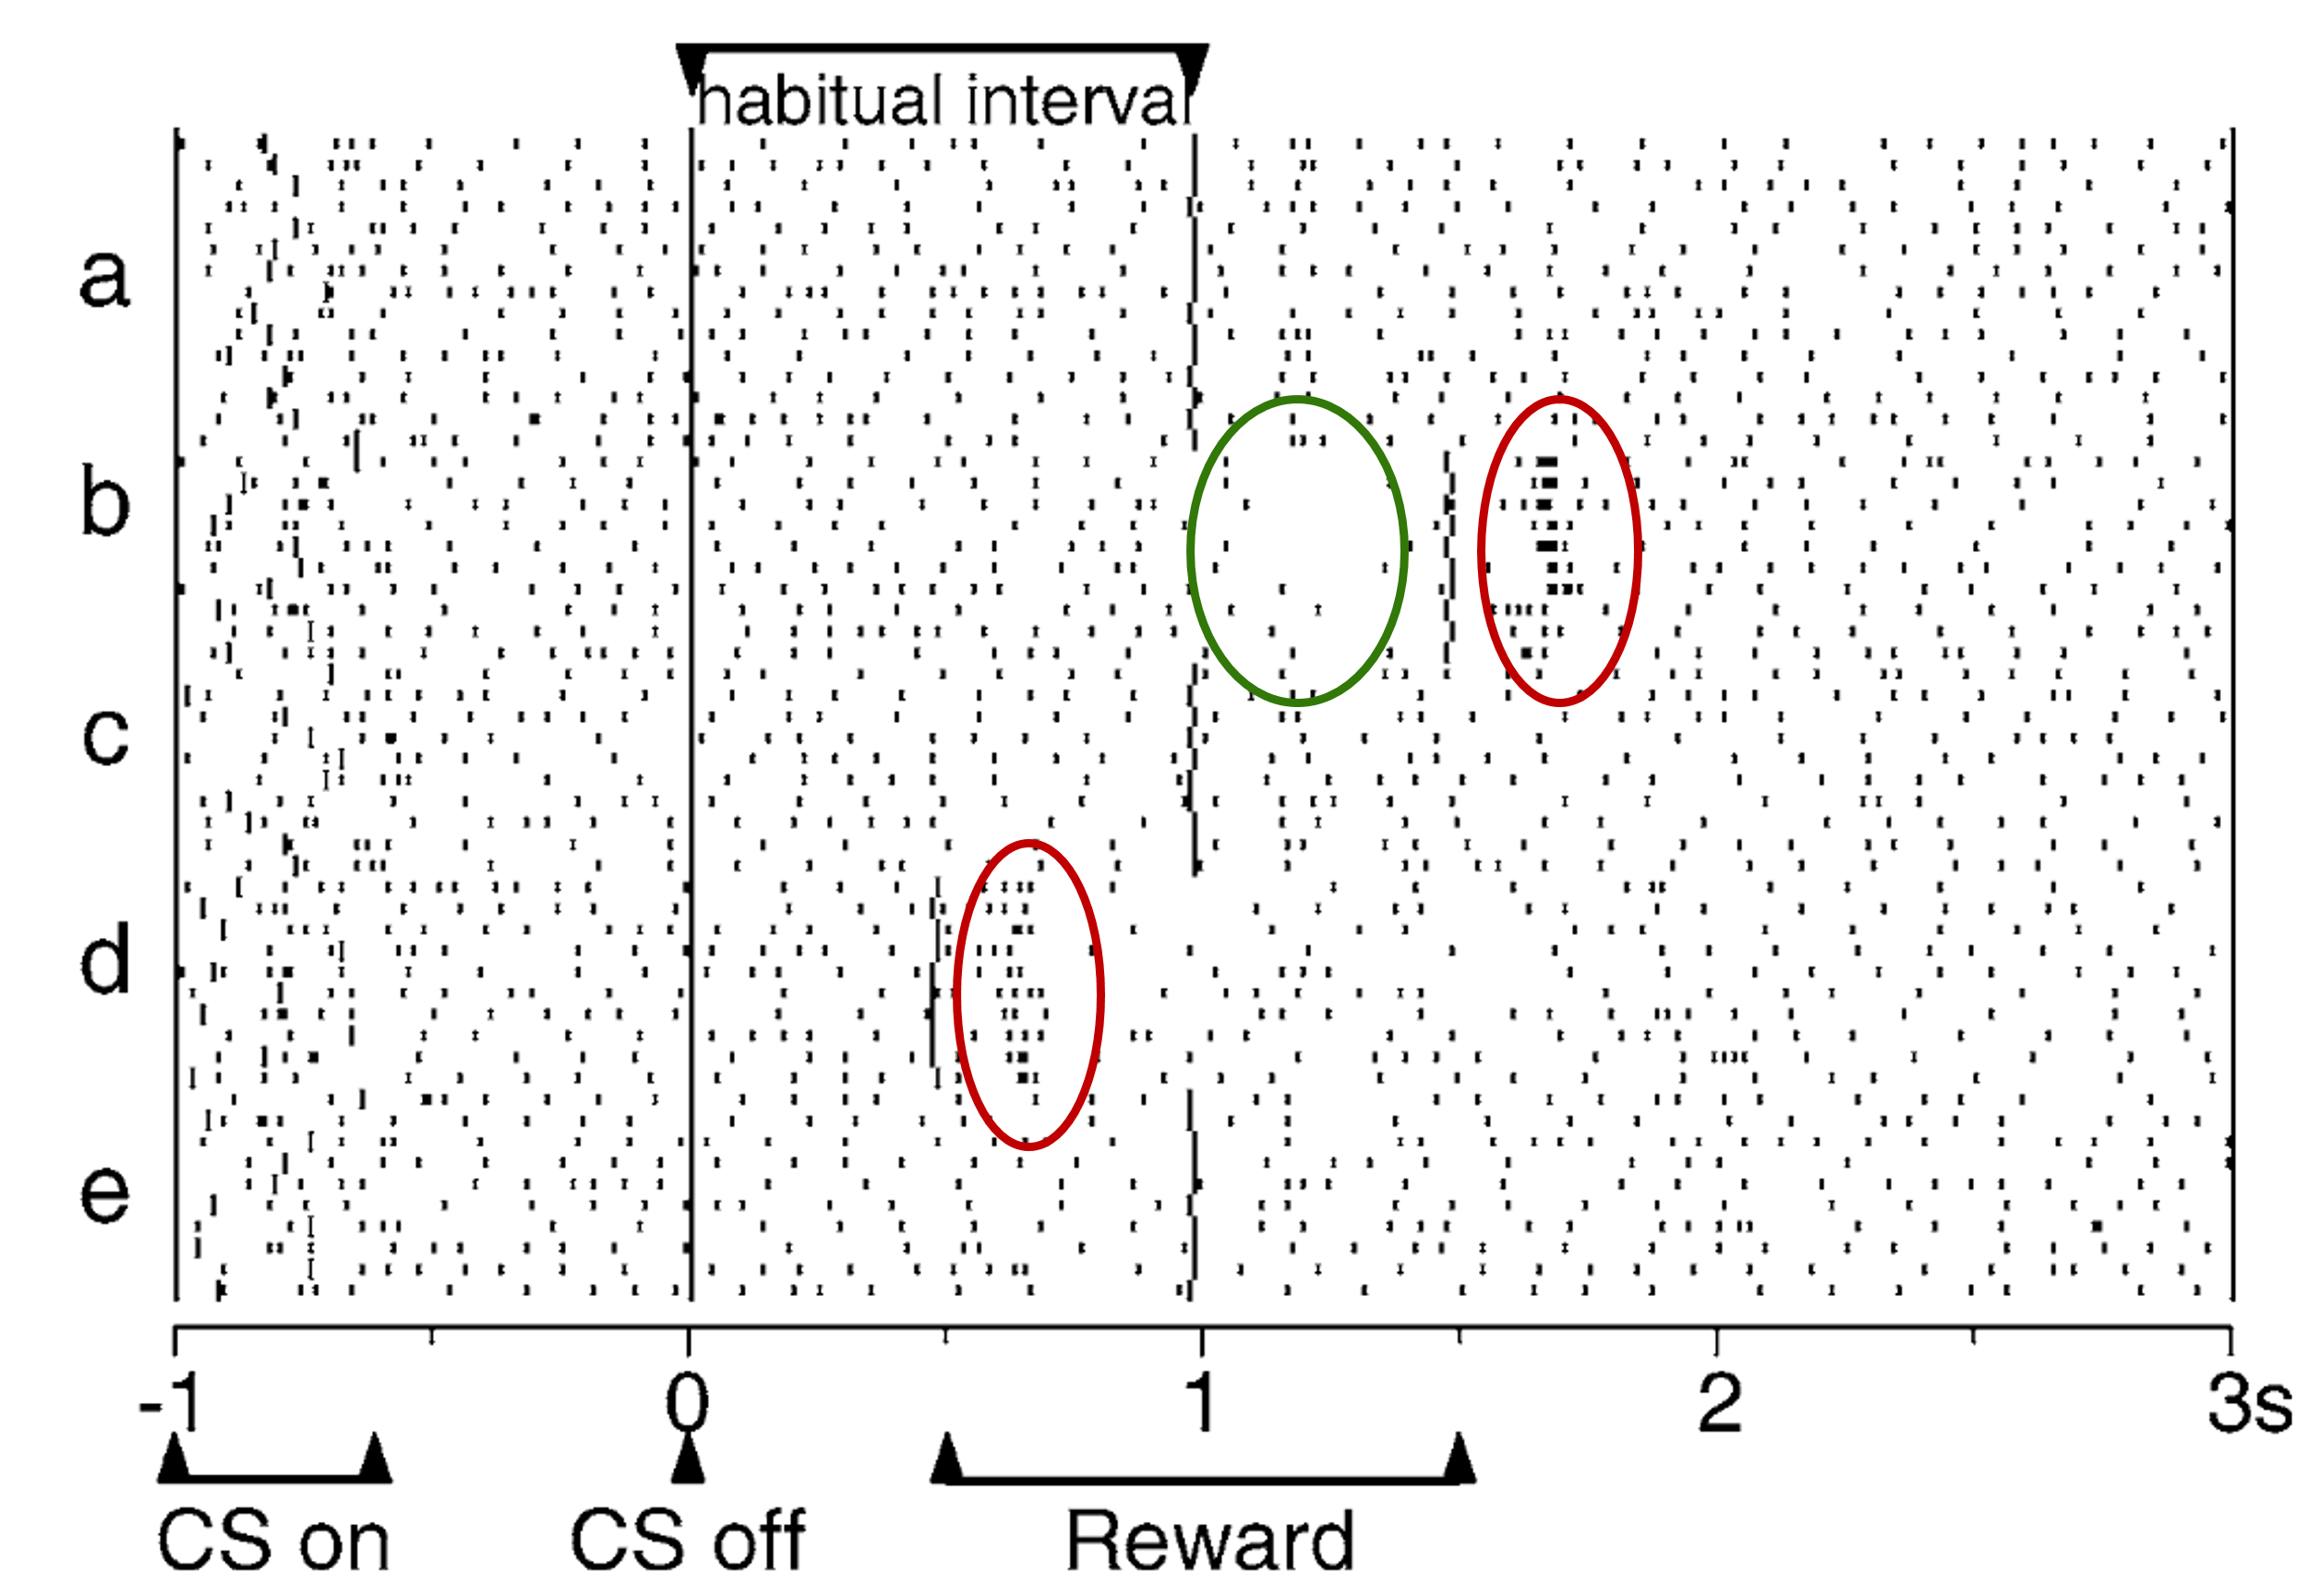
\includegraphics[width=0.5\linewidth]{./img/dopamine_timing.png}
            \end{center}
        \end{casestudy}
\end{description}

\begin{remark}
    Dopamine is therefore a signal for the predicted error and not strictly for the reward.
\end{remark}